\chapter{Zugriffs-Möglichkeiten auf eine Domino-Datenbank}



Um Anwendungen welche sich auf dem Domino-Server befinden auszuführen, gibt es mehrere Möglichkeiten.
In diesem Kapitel werden diese Zugriffsarten behandelt.\newline

%Eine Anwendung welche im Domino Administrator erstellt wurde, kann auf unterschiedliche Arten aufgerufen und bearbeitet werden.


\section{Client Zugriff}
\label{sec:5webzugriff}

%buch --> ebel s.30 für client!!!!!!!
Im Gegensatz zu Lotus Domino stellt Lotus Notes die Seite des Client dar. Der Notes Client verwaltet die Benutzeroberfläche und ist für die grafische Aufbereitung
der Daten zuständig.\newline
Notes Clients interagieren mit Datenbanken, welche sich am Domino-Server befinden, in unterschiedlicher Weise.
Grundsätzlich gibt es zwei mögliche Zugriffsarten:
\begin{itemize}
\item Zugriff mit Notes Client 
\item Zugriff über einen Web-Browser, zum Beispiel mit Internet Explorer oder Mozilla Firefox 
\end{itemize}



\subsection{Zugriff über Notes Client}
\label{sec:5webzugriff}

Für die Kommunikation eines Notes Client mit einem Domino Server werden Protokolle benötigt. Diese Kommunikation wird entweder über Notes-Protokolle
(NRPC) oder über Internet-Protokolle wie POP3 oder IMAP abgewickelt (Kapitel 2.3.1).
Der Anwender greift dabei auf Datenbanken, auf die er die Zugriffsberechtigung besitzt, zu. 
Diese Datenbanken werden als Datenbanksymbole auf dem
Arbeitsplatz im Notes Client abgelegt\cite{ebel}.

\begin{figure}[H]
    \centerline{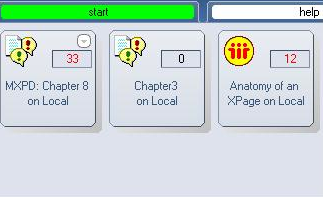
\includegraphics[scale=0.5]{pics/Client_kacheln}}
    \caption[Darstellung einer Datenbank im Notes Client]{\label{FiG:Darstellung einer Datenbank im Notes Client}
	In dieser Abbildung ist die Darstellung von drei Datenbanken, als Datenbanksymbole im Notes Client ersichtlich.}
\end{figure}



to do....%S.31 ebel!!!

%Möchte man eine Anwendung, wie zum Beispiel das erstellte Template, vom Notes-Client aus starten, geht dies wie folgt von statten. Wie in Kapitel 2.3 erwähnt
%handelt es sich bei Lotus/Domino um eine Anwendung die in einer Server/Client Architektur operiert. Das bedeutet verfügbaren Datenbanken sind auf einem 
%oder mehreren Servern abgelegt. Diese Datenbanken können mit dem Notes Client geöffnet und bearbeitet werden. 
%Dabei handelt es sich um Datenbanken mit einer \textit{.nsf}-Endung. Diese Endung steht für Notes Storage Facility.\\

%Wird eine Anwendung vom Server gestartet, wird eine automatische Verknüpfung mit der Oberfläche des Clients erstellt. 

\subsection{Zugriff über Web-Browser}
\label{sec:5webzugriff}

Um den Zugriff über einen Browser zu ermöglichen, wird vorausgesetzt, dass sich die Anwendung auf einem Domino-Server befindet, welcher als Webserver
agiert\cite{ebel}.
Die eindeutige Adresse eines Ressource oder eines Dokuments im Internet bezeichnet man als URL (Uniform Ressource Locator). Eine URL setzt sich aus 
bestimmten syntaktischen Regeln zusammen. Diese Regeln enthalten unter anderem den Namen des Host-Rechners und den Pfad beziehungsweise
den Namen des Dokuments\cite{knaepper}.\\
Die URL kann sich zum Beispiel wie folgt zusammensetzten:
\begin{equation}
http://s124/work/template.nsf/default.xsp
\end{equation} 

In diesem Beispiel wird eine XPage, namens \textit{default}, aufgerufen. Diese XPage ist ein Teil der Datenbank \textit{template}, \textit{work} ist das
Verzeichnis auf dem Server \textit{s124}, der zu diesem Dokument führt. Hierbei handelt es sich um einen Webserver welcher, Hypertext Transfer Protocol
(HTTP) zum Informationsaustausch benutzt. Das hier angeführte Beispiel, beschränkt sich auf den lokalen Zugriff über das Intranet.\newline
 Wird der Zugriff über das Internet durchgeführt, so setzt sich die URL wie folgt zusammen.
\begin{equation}
http://server.domain.com/work/template.nsf/default.xsp
\end{equation} 


Die sich auf dem Server befindenden Datensätze, können auch von einen Webbrowser aufgerufen werden. 
 to do....

%Die Aufgabe eines Web-Servers besteht im allgemeinen darin, aus einer URL die entsprechende Datei......


%knaepper kapitel 31
%Hierfür wurde das Template
%Auch auf das erstellte Template kann vom Notes-Client oder einen Web-Browser geöffnet werden.

%================================

%\subsection{Ansichten und Ordner im Web}
%\label{sec:5webzugriff}

%\subsection{XPages und Custom Controls im Web}
%\label{sec:5webzugriff}
